\section{Background}
Amidakuji is a custom in Japan which 
allows for a pseudo-random assignment of children to prizes\cite{A1}. 
Usually done in Japanese schools, a teacher will draw $N$ vertical lines, 
hereby known as lines, where $N$ is the number of students in class. 
At the bottom of each line will be a unique prize. At the top of each line will be the name of one of the students.  
The teacher will then draw 0 or more horizontal lines, hereby known as \emph{bars}, 
connecting two adjacent lines. The more bars there are the more complicated (and fun) 
the Amidakuji is. No two endpoints of two bars can be touching. Each student then traces 
their line, and whenever they encounter an end point of a bar along their line, 
they must cross the bar and continue going down the adjacent line. 
The student continues tracing down the lines and crossing bars 
until they get to the end of the ladder lottery. The prize at the bottom of the ladder lottery 
is their prize\cite{A1}. See Fig.\ref{fig:aa} for an example of a ladder lottery.\par
The word Amidakuji has an interesting etymology. In Japanese, Amida is the Japanese name 
for Amithaba, the supreme Buddha of the Western Paradise. Amithaba
was a Buddha from India and there was a cult based around him. The cult 
of Amida, otherwise known as Amidism, believed that by worshiping Amithaba, they would 
enter into the his Western Paradie\cite{A0}. Amidism began in India in the fourth century,
made its way to China and Korea in the fifth century, and finally  came 
to Japan in ninth century \cite{A0}. It was in Japan where the game Amidakuji
began. It is known as 'Ghost Legs' in China and Ladder Lotteries in English.\par
The game Amidakuji began in Japan in the Muromachi period, which spanned from
1336 to 1573\cite{A0}. During the Muromachi period, the game was played by having
players draw their names at the top of the lines, and at the bottom 
of the lines were pieces of paper that had the amount the players
were willing to bet. The pieces of paper were folded in the shape of 
Amithaba's halo, which is why the game is called Amidakuji. Kuji 
is the Japanese word for lottery. Hence the name of the game being 
Amidakuji.\par 

An interesting property about ladder lotteries is that they can be derived from a 
\emph{permutation} which is a is a unique ordering of objects\cite{A1}.
For the purposes of this paper, the objects of a permutation will be integers 
ranging from [$1$ $\dots$ $N$]. \emph{Optimal ladder lotteries} are a special case of ladder 
lotteries in which there is one bar in the ladder for each \emph{inversion} in the permutation\cite{A1}.
An \emph{inversion} is a relation between two elements in $\pi$, 
$\pi_{i}$ and $\pi_{j}$, such that if $\pi_{i}>\pi_{j}$ and $i<j$ then $\pi_{i}$ and $\pi_{j}$ 
form an inversion. 
For example, given $\pi=(4,3,5,1,2)$, its iversion set is $Inv\{\pi\} =\{(4,3),(4,1),(4,2),(3,1),(3,2),(5,1),(5,2)\}$.
Every permutation has a unique, finite set of optimal ladder lotteries associated with it. 
 Thus, the set of optimal ladder lotteries associated with $\pi$, 
 hereby known as \emph{$OptL\{\pi\}$}, is the set containing all ladder lotteries 
 with a number of bars equal to the number of inversions in $\pi$. 
 See Fig.\ref{fig:ab} for an example of an optimal ladder in $OptL\{(4,3,2,1)\}$.
 For each optimal ladder in $OptL\{\pi\}$, the $N$ 
 elements in $\pi$ are listed at the top of a ladder and each 
 element is given its own line. 
 At the bottom of a ladder is the \emph{sorted permutation}, 
 hereby known as the \emph{identity permutation}\cite{A1}. 
 The  identity permutation of size $N$ is defined as follows - $I:(1, 2, 3, \dots, N)$. 
 Each ladder in $OptL\{\pi\}$ has the minimal number of bars to sort $\pi$ 
 into the identity permutation. Each bar in a ladder from $OptL\{\pi\}$ uninverts a single 
 inversion in $\pi$ exactly once. For the remainder of this paper, only optimal ladder 
 lotteries will be discussed, with one exception. Therefore, when the term ladder lottery is used, assume 
 optimal ladder lottery unless otherwise stated. The foundational data structures used to perform the research in this thesis are the following. 
 Let the \emph{ladder} be a two dimensional 
array. Let $\pi_{N}$ be some arbitrary permutation of order $N$. The ladder has $k$ rows where $0 \leq k \leq N(N-1)/2$. 
The ladder has $N-1$ columns.  
\begin{figure}[!htp]
	\begin{minipage}{0.4\textwidth}
		\centering
		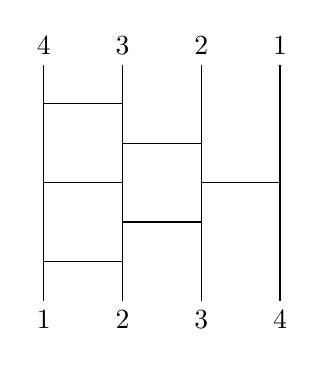
\begin{tikzpicture}
		 	\draw(0, 0) to (0, 3) ++(0, 0) node[above]{4} --(0, 0)node[below]{1};
		 		\draw(0, 2.5) to (1, 2.5);
		 		\draw(0, 1.5) to (1, 1.5);
		 		\draw(0, 0.5) to (1, 0.5);

		 	\draw(1, 0) to (1, 3) ++(0, 0) node[above]{3} --(1, 0)node[below]{2};
		 		\draw(1, 2) to (2, 2);
		 		\draw(1, 1) to (2, 1);
		 	\draw(2, 0) to (2, 3) ++(0, 0) node[above]{2} --(2, 0)node[below]{3};
		 		\draw(2, 1.5) to (3, 1.5);
		 	\draw(3, 0) to (3, 3) ++(0, 0) node[above]{1} --(3, 0) node[below]{4};
		\end{tikzpicture}
				

	\end{minipage}
	\begin{minipage}{.4\textwidth}
		\begin{flushright}
		
		
		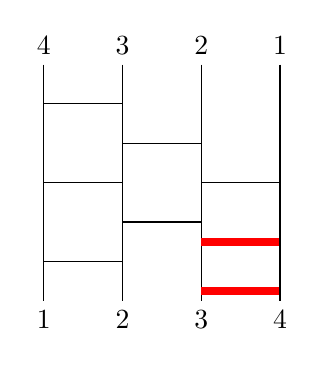
\begin{tikzpicture}
		 	\draw(0, 0) to (0, 3) ++(0, 0) node[above]{4} --(0, 0)node[below]{1};
		 		\draw(0, 2.5) to (1, 2.5);
		 		\draw(0, 1.5) to (1, 1.5);
		 		\draw(0, 0.5) to (1, 0.5);
		 		

		 	\draw(1, 0) to (1, 3) ++(0, 0) node[above]{3} --(1, 0)node[below]{2};
		 		\draw(1, 2) to (2, 2);
		 		\draw(1, 1) to (2, 1);
		 	\draw(2, 0) to (2, 3) ++(0, 0) node[above]{2} --(2, 0)node[below]{3};
		 		\draw(2, 1.5) to (3, 1.5);
		 		\draw[line width=1mm, red](2, 0.75) to (3, 0.75);
		 		\draw[line width=1mm, red](2, 0.125) to (3, 0.125);
		 	\draw(3, 0) to (3, 3) ++(0, 0) node[above]{1} --(3, 0) node[below]{4};
		\end{tikzpicture}
	\end{flushright}
	\end{minipage}
	\caption{Two ladders for the permutation (4, 3, 2, 1). The left ladder is an optimal ladder and the right ladder is not. Therefore the left ladder belongs to $optL\{(4,3,2,1)\}$. The bold  bars in the right ladder are redundant, thus the right ladder is not optimal}
	\label{fig:ab}
\end{figure}

%%FUCKING LATEX.....


%%\centerline{
\includegraphics[width=10cm,height=5cm,keepaspectratio]{Buddha}}



\begin{center}
\begin{figure}[!htp]
		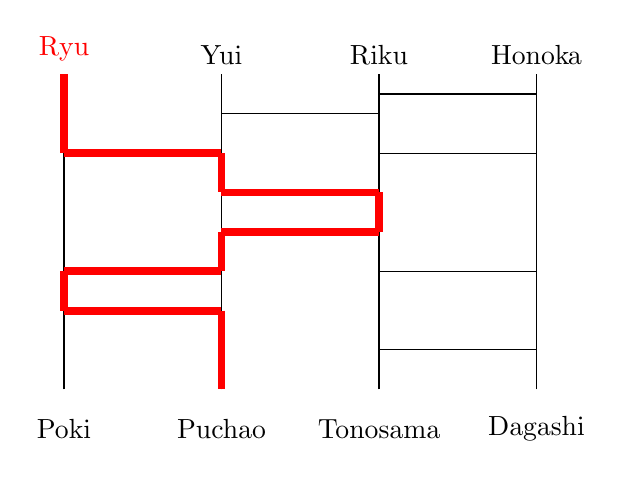
\begin{tikzpicture}
		%%Start of figure. Fig 1
			\draw(0, 0) to (0, 3); 
		
			\node at (0, -0.5){Poki};
			\draw(2, 0) to (2, 4) node[above]{Yui};
			\node at (2, -0.5){Puchao};
			\draw(4, 0) to (4, 4)node[above]{Riku};
			\node at (4, -0.5){Tonosama};
			\draw(6, 0) to (6, 4)node[above]{Honoka};
			\node at (6, -0.5){Dagashi};
			
			%bars%
		    \draw[line width=1mm, red](0, 3) to (0, 4) node[above]{Ryu};
			\draw[line width=1mm, red](0, 1) to (2, 1);
			\draw[line width=1mm, red](2, 1.5) to (2, 2);
			\draw[line width=1mm, red](0, 1)to(0, 1.5);
			\draw[line width=1mm, red](2, 1) to (2, 0);
			\draw[line width=1mm, red](0, 3) to (2, 3);
			\draw[line width=1mm, red](2, 3) to (2, 2.5);
			\draw[line width=1mm, red](4, 2) to (4, 2.5);
			\draw[line width=1mm, red](0, 1.5) to (2, 1.5);
			
			\draw[line width=1mm, red](2, 2) to (4, 2);
			\draw[line width=1mm, red](2, 2.5) to (4, 2.5);
			\draw(2, 3.5) to (4, 3.5);
			
			\draw(4, 0.5) to (6, 0.5);
			\draw(4, 3) to (6, 3);
			\draw(4, 1.5) to (6, 1.5);
			\draw(4, 3.75) to (6, 3.75);
		\end{tikzpicture}
\caption{A ladder lottery where Ryu gets Puchao, Yui gets Dagashi, Riku gets Tonosama and Honoka gets Poki. You can see that Ryu's path is marked by red bars.}
\label{fig:aa}
\end{figure}
\end{center}


\section{Thesis Statement}
  	This thesis provides full, or partial, solutions to two problems related 
    to ladder lotteries. The first problem is the so called canonical ladder listing problem. 
    This problem asks, given all $N!$ permutations of order $N$, is there an algorithm 
    to list a canonical ladder from each permutation's $OptL\{\pi\}$? In other words, 
	is there an easy way to transition from a ladder in 
	a given $OptL\{\pi\}$ to the next ladder in the next $OptL\{\pi\}$ until all $N!$ $OptL\{\pi\}$ have had a canonical 
	ladder represented?  This thesis provides two such algorithms for solving the canonical 
	listing problem. The second problem is the so called minimum height 
    problem which asks, given all the ladders in $Optl\{\pi\}$, which ladder(s) are 
    the shortest? That is to say, which ladders have the least number of rows? Furthermore, given some arbitrary $\pi$, 
    is there a way to create a ladder for $\pi$ with minimal height? This thesis 
    provides an upper and lower bound for the minimal height of ladders along with a heuristic algorithm 
	for creating a ladder with minimal height.
	
\section{Overview of Thesis}
This thesis is broken down into several sections. Firstly, a literature 
review of ladder lotteries will be provided. The literature review focuses on solved problems pertaining 
to ladder lotteris along with the commonalities between ladder lotteries and 
other mathematical objects. Following the literature review, two chapters pertaining to the two problems will be 
provided. In each of these chapters there is an introduction to the problem, a methodology section, a results 
section and a conclusion section. The introduction section introduces the problem to the reader, providing the necessary 
definitions and concepts. The methodology sections contain the algorithms and formulas used to solve the respective problems. 
Following the methodology sections, the results generated by the algorithms will be presented.
In the results sections there will be proofs and formulas for certain propositions made in regards to the respective problems. 
Following the results section, an analysis of the results will be presented along with a summary of future work. In this section,
the failures and successes of this research will be analyzed. There will also be commentary on 
open (unsolved) problems related to ladder lotteries and a 
discussion of how research on ladder lotteries could be used in other fields.
Finally, a conlcusion that summarizes the thesis will be provided.